\documentclass[a4paper]{article}
\usepackage[margin=1in]{geometry}
\usepackage{graphicx} % Required for inserting images
\usepackage[french]{babel}

\usepackage{hyperref}
\usepackage{listings}
\usepackage{xcolor}
\usepackage[settings]{markdown}
\usepackage{fancyvrb}  % pour verbatim, affichage brut de texte
\usepackage{amsthm}
\theoremstyle{theorem}
\usepackage{graphicx}
\usepackage{float}
 \newtheorem{theorem}{Theorem}[section]
\theoremstyle{definition}
\newtheorem{definition}{Definition}[section]
\usepackage{tikz}


\lstset{
    language=C,
    basicstyle=\ttfamily\small,
    keywordstyle=\color{blue}\bfseries,
    stringstyle=\color{red},
    commentstyle=\color{green!50!black}\itshape,
    morecomment=[l][\color{magenta}]{\#},
    numbers=left,
    numberstyle=\tiny\color{gray},
    stepnumber=1,
    numbersep=5pt,
    backgroundcolor=\color{black!5},
    frame=single,
    rulecolor=\color{black!30},
    tabsize=4,
    captionpos=b,
    breaklines=true,
    breakatwhitespace=false,
    title=\lstname,
    showstringspaces=false
}


\title{TER :  Découverte et implémentation de systèmes de preuves 0-knowledge.}
\author{Raphael LEONARDI}
\begin{document}

\maketitle

\section{Introduction}

J'effectue un TER au sein de l'INRIA, dans l'équipe GRACE, dans le but de découvrir et d'implémenter des systèmes de preuves 0-knowledge. Pour cela, j'utilise le langage C et plus précisémment la bibliothèque PARI GP.

\vspace{1cm}
La Zero Knowledge Proof ou preuve à divulgation nulle de connaissance est un protocole permettant à un utilisateur de prouver qu'une situation est réelle sans avoir à révéler d'information relative à cette dernière. Il s'agirait par exemple pour une personne de prouver son identité sans avoir à la révéler.

\vspace{1cm}
Les protocoles de preuve 0-Knowledge se base sur des interactions entre deux acteurs : le prouveur et le vérifieur.  
Le prouveur va essayer de convaincre le vérifieux qu'il connait les information, sans les lui révéler au début, et le vérifieur va chercher à vérifier l'honnêteté du prouveur.

\section{Implémentation en C d'un groupe}
On aura besoin au cours de ce projet d'utiliser des groupes en C, en utilisant la bibliothèque Pari GP. Voici comment j'ai défini ce qu'était un groupe en C :
\begin{lstlisting}
typedef enum  {
    ADD = 0,
    MUL = 1
} loiComp;


// On definit ce qu est une loi de groupe
// C est a dire une fonction prennant GEN x, GEN y
// Et renvoyant une loi de groupe dessus ()
// Une loi est une fonction de signature (GEN, GEN) -> GEN
typedef GEN (*Loi)(GEN, GEN);

typedef struct{
    Loi mul;
    GEN one;
} Group;

\end{lstlisting}
On a crée un typé énuméré pour la loi de composition pour utiliser des groupes tels que $(Z/nZ)$.
\section{Première Implémentation d'un algorithme sur des groupes} 

Pour commencer j'ai effectué une première implémentation de preuves en me basant sur la méthode décrite dans l'article page 16.
\href{https://www.google.com/url?sa=t&rct=j&q=&esrc=s&source=web&cd=&cad=rja&uact=8&ved=2ahUKEwjUgo7fqsOLAxWkfKQEHaJBHLMQFnoECBYQAQ&url=https%3A%2F%2Feprint.iacr.org%2F2017%2F1066.pdf&usg=AOvVaw3hDT__ZU-Hu_KgOIIbMhYM&opi=89978449}{ Bulletproofs: Short Proofs for Confidential Transactions and More}
\vspace{0.5cm}
J'ai choisi d'implémenter le prouveur et le vérifieur comme étant des structures en C, comme définis ici dans ce fichier .h : 
\begin{lstlisting}

typedef enum {
    REJECT = 0,
    ACCEPT = 1
} result;

typedef struct{
    GEN g;
    GEN h;
    GEN u;
    GEN P;
    GEN a;
    GEN b;

    Group *groupe;

} prover;

typedef struct{
    GEN g;
    GEN h;
    GEN u;
    GEN P;
    Group *groupe;


} verifieur;

\end{lstlisting} 

\subsection{But de l'Algorithme}
L'algorithme fonctionne sur une structure de groupe $G$ d'on  on connaît des générateurs  $g,h$ ($g$ et $h$ contiennent chacune des générateurs). Ces générateurs $g$ et $h$ sont les entrées de l'algorithme, ainsi que $P \in G$ et $c$ un scalaire $\in (Z/pZ)$ avec $p$ premier.

\vspace{0.5cm}
Le but du prouveur sera de convaincre le vérifieur qu'il connait deux vecteurs $a,b \in Z^{n}$ tels que : 
\label{key}\[P = g^a h^b    \quad et \quad c=⟨a,b⟩\]


Pour cela, on va introduire  un élément u, $\in$ G. On va calculer $c=⟨a,b⟩$. Pour vérifier que le produit scalaire est validé, on va plutôt vérifier que :

\[ P =g^a h^b u^c \]

\subsection{Entrées et sorties de l'algorithme}

Soit $p$ un nombre premier, et $n = 2^k, k \in N$.

Entrées : $g, h \in G^{n}, u, P\in  G, a, b\in \mathbb{Z}_{p}^{n} $


Entrée prouveur P : $g,h,a,b,u,P$

Entrée vérifieur V : $g,h,u,P$

Sortie :  ACCEPT ou REJECT


\subsection{Etapes de l'algorithme}


Voici l'algorithme tel qu'il est défini dans l'article :




   
    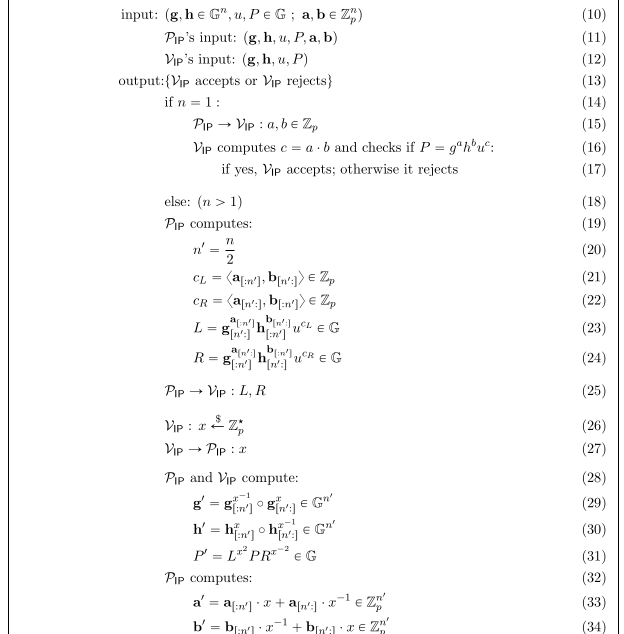
\includegraphics[width=1\linewidth]{proofPro.png}

\subsection{Implémentation de l'algorithme en langage C : }
L'algorithme est récursif, à chaque itération on divise la taille des paramètres $g,h$ par 2 , jusqu'à arriver à 1, au cas de base. On doit faire la vérification dans ce cas base, voila comment j'ai décidé de l'implémenter en C : 

\begin{lstlisting}
    
/*La partie finale de la preuve*/
result check(verifieur *v,GEN a, GEN b,GEN g, GEN h, GEN P){
    /*Calcule dans un premier temps c*/

    
    GEN c = dot(a, b);
    
    Loi mul = v->groupe->mul;


    /*On calcule g^a *h^b *u^c */
    GEN gauche = powerVector(v->groupe, g, a);
   
    GEN droite = powerVector(v->groupe, h, b);
    GEN fin = power(v->groupe, v->u, c);

    GEN prod = mul(gauche, mul(droite,fin));
    /*On verifie que prod  egal a P*/

    // intResult transforme un entier en ACCEPTED ou REJECTED
    return intResult(gequal(prod, P));

}

\end{lstlisting}
Quand à la partie récursive, on doit recalculer des éléments $g,h$ comme ceci :
  \begin{lstlisting}
    GEN leftRight = proverfirstComputation(bob, a, b, g, h);
    GEN L = gel(leftRight, 1); GEN R = gel(leftRight, 2);

    GEN x = verifierChooseX(p);
    GEN common = computationCommon(bob->groupe, L, R, P, g, h, x);
    GEN g2 = gel(common, 1); GEN h2 = gel(common, 2); GEN P2 = gel(common, 3);

    GEN ab = proversecondComputation(bob,a,b ,x );

    GEN a2 = gel(ab, 1); GEN b2 = gel(ab, 2);
      
    return protocolRecursive(bob, alice,g2, h2, u, P2, a2, b2 ,n/2,p);

  \end{lstlisting}

On a utilisé plusieurs sous fonctions dans la partie récursive :

\begin{enumerate}
    \item $proverfirstComputation()$ qui calcule les éléments $L$ et $R$ décrits dans l'algorithme pour le prouveur uniquement.
    \item $verifierChooseX()$ qui prend en argument un nombre entier et renvoie un élément au hasard dans $(Z/pZ)^*$. Attention ici p doit être premier, en effet si p ne l'était pas, l'élément $x^{-1}$ n'aurait pas de garantie d'exister.
    \item $computationCommon()$ qui est faite par le vérifieur et le prouveur, et qui calcule les valeurs de $g$ et $h$ pour la prochaine itération.
    \item $proverSecondComputation()$ qui est calculée par le prouveur, et qui calcule les valeurs de $a$ et $b$ pour la prochaine itération.
\end{enumerate}

Ensuite on lance l'appel récursif sur les nouveaux paramètres, jusqu'à atteindre le cas de base.


\section{Utilisation de l'algorithme sur un exemple}
Maintenant que l'on a implémenté nôtre algorithme en C, il faut maintenant pouvoir le tester sur des vraies valeurs.
\subsection{Obtenir $P$ et en fonction de $g,h,a,b,u$}
Le proveur essaie de convaincre le vérifieur qu'il connait $a,b$ qui vérifient l'égalité. Pour pouvoir tester notre fonction, on a besoin d'obtenit P en fonction des paramètres $g,h,a,b,u$, que l'on obtient par la fonction suivante en C :
\begin{lstlisting}
    GEN buildP(Group *G, GEN g, GEN h, GEN a, GEN b, GEN u){
  GEN G2 = powerVector(G, \left( g, a);
  GEN c = dot(a, b);
  GEN G3 = powerVector(G ,h, b);
  GEN G4 = powerVector(G, u, c);
 

  return G->mul(G2, G->mul(G3, G4));

}

\end{lstlisting}
\subsection{Exemple}
Maintenant que l'on a l'algorithme, et les bonnes valeurs, on peut enfin s'en servir sur un exemple.\\
Prennons le groupe $G = (Z/pZ, +)$ , avec p un nombre premier. Ici on va d'abord se concentrer sur des petits nombres pour pouvoir trouver les erreurs facilement si il y en a. Voici les valeurs que l'on prendra : 
\[p = 17, G = (Z/17Z, +), n = 8,  u =\overline{10}, P = \overline{12}\]

 \[g=[\overline{4}, \overline{5}, \overline{7}, \overline{8}, \overline{9}, \overline{12}, \overline{13}, \overline{15} ],h = [\overline{7} ,\overline{2} ,\overline{3} ,\overline{4} ,\overline{12} ,\overline{1} ,\overline{14} ,\overline{16} ], a = [\overline{4} ,\overline{5} ,\overline{6} ,\overline{2} ,\overline{1} ,\overline{5} ,\overline{9} ,\overline{15} ] , b = [\overline{3} ,\overline{7} ,\overline{8} ,\overline{16} ,\overline{4} ,\overline{3} ,\overline{2} ,\overline{7}]\]

 J'ai ajouté un affichage, qui affichent les valeurs calculées par le vérifieur et le prouveur. Si l'on redirige le dans un Markodwn, on obtient un joli visuel. Voici ce que l'affichage a donnée pour cet exemple : 

\begin{Verbatim}[frame=single, fontsize=\scriptsize]
Lancement protocole avec n = 8 et p = 17
-----------------------------------------
## Appel recursif avec n = 8
-     a = [Mod(4, 17), Mod(5, 17), Mod(6, 17), Mod(2, 17), Mod(1, 17), Mod(5, 17), Mod(9, 17), Mod(15, 17)]
-     b = [Mod(3, 17), Mod(7, 17), Mod(8, 17), Mod(16, 17), Mod(4, 17), Mod(3, 17), Mod(2, 17), Mod(7, 17)]
-     g = [Mod(4, 17), Mod(5, 17), Mod(7, 17), Mod(8, 17), Mod(9, 17), Mod(12, 17), Mod(13, 17), Mod(15, 17)]
-     h = [Mod(7, 17), Mod(2, 17), Mod(3, 17), Mod(4, 17), Mod(12, 17), Mod(1, 17), Mod(14, 17), Mod(16, 17)]  
Le prouveur a calcule L  = Mod(9, 17) et R = Mod(9, 17)  
Le verifieur a choisi x = Mod(7, 17)  
 Les calculs en communs on ete effectues.  
Le prouveur et le verifieur ont calcule :   
-      g' = [Mod(15, 17), Mod(7, 17), Mod(7, 17), Mod(9, 17)] 
-      h' = [Mod(7, 17), Mod(2, 17), Mod(6, 17), Mod(6, 17)] 
-      P' = Mod(15, 17)
-----------------------------------------
## Appel recursif avec n = 4
-     a = [Mod(16, 17), Mod(9, 17), Mod(2, 17), Mod(4, 17)]
-     b = [Mod(9, 17), Mod(5, 17), Mod(3, 17), Mod(10, 17)]
-     g = [Mod(15, 17), Mod(7, 17), Mod(7, 17), Mod(9, 17)]
-     h = [Mod(7, 17), Mod(2, 17), Mod(6, 17), Mod(6, 17)]  
Le prouveur a calcule L  = Mod(16, 17) et R = Mod(12, 17)  
Le verifieur a choisi x = Mod(5, 17)  
 Les calculs en communs on ete effectues.  
Le prouveur et le verifieur ont calcule :   
-      g' = [Mod(4, 17), Mod(9, 17)] 
-      h' = [Mod(9, 17), Mod(1, 17)] 
-      P' = Mod(0, 17)
-----------------------------------------
## Appel recursif avec n = 2
-     a = [Mod(9, 17), Mod(5, 17)]
-     b = [Mod(10, 17), Mod(0, 17)]
-     g = [Mod(4, 17), Mod(9, 17)]
-     h = [Mod(9, 17), Mod(1, 17)]  
Le prouveur a calcule L  = Mod(13, 17) et R = Mod(3, 17)  
Le verifieur a choisi x = Mod(12, 17)  
 Les calculs en communs on ete effectues.  
Le prouveur et le verifieur ont calcule :   
-      g' = [Mod(12, 17)] 
-      h' = [Mod(16, 17)] 
-      P' = Mod(13, 17)
-----------------------------------------
## Verification finale sur  :  
     a = [Mod(5, 17)]  
     b = [Mod(15, 17)]  
     g = [Mod(12, 17)]  
     h = [Mod(16, 17)]  
     u = Mod(10, 17)  
     P = Mod(13, 17)  
     Verdict verifieur : ACCEPT

\end{Verbatim}

Dans cet exemple, le vérifieur a accepté les arguments du prouveur, les valeurs sont bonnes. Maintenant voici ce qui se passe si l'on change des valeurs quelconque dans a et b, qui rendront fausses les conjectures. Prennons comme nouvelles valeurs  de a et b: 
 \[ a = [\overline{1} ,\overline{5} ,\overline{2} ,\overline{2} ,\overline{1} ,\overline{5} ,\overline{9} ,\overline{15} ] , b = [\overline{3} ,\overline{7} ,\overline{8} ,\overline{16} ,\overline{2} ,\overline{3} ,\overline{2} ,\overline{7}]\]
On obtient ce résultat : 
 \begin{Verbatim}[frame=single, fontsize=\scriptsize]
     Lancement protocole avec n = 8 et p = 17
-----------------------------------------
## Appel recursif avec n = 8
-     a = [Mod(1, 17), Mod(5, 17), Mod(2, 17), Mod(2, 17), Mod(1, 17), Mod(5, 17), Mod(9, 17), Mod(15, 17)]
-     b = [Mod(3, 17), Mod(7, 17), Mod(8, 17), Mod(16, 17), Mod(2, 17), Mod(3, 17), Mod(2, 17), Mod(7, 17)]
-     g = [Mod(4, 17), Mod(5, 17), Mod(7, 17), Mod(8, 17), Mod(9, 17), Mod(12, 17), Mod(13, 17), Mod(15, 17)]
-     h = [Mod(7, 17), Mod(2, 17), Mod(3, 17), Mod(4, 17), Mod(12, 17), Mod(1, 17), Mod(14, 17), Mod(16, 17)]  
Le prouveur a calcule L  = Mod(2, 17) et R = Mod(9, 17)  
Le verifieur a choisi x = Mod(2, 17)  
 Les calculs en communs on ete effectues.  
Le prouveur et le verifieur ont calcule :   
-      g' = [Mod(3, 17), Mod(1, 17), Mod(4, 17), Mod(0, 17)] 
-      h' = [Mod(3, 17), Mod(13, 17), Mod(13, 17), Mod(16, 17)] 
-      P' = Mod(1, 17)
-----------------------------------------
## Appel recursif avec n = 4
-     a = [Mod(11, 17), Mod(4, 17), Mod(0, 17), Mod(3, 17)]
-     b = [Mod(14, 17), Mod(1, 17), Mod(8, 17), Mod(5, 17)]
-     g = [Mod(3, 17), Mod(1, 17), Mod(4, 17), Mod(0, 17)]
-     h = [Mod(3, 17), Mod(13, 17), Mod(13, 17), Mod(16, 17)]  
Le prouveur a calcule L  = Mod(6, 17) et R = Mod(10, 17)  
Le verifieur a choisi x = Mod(2, 17)  
 Les calculs en communs on ete effectues.  
Le prouveur et le verifieur ont calcule :   
-      g' = [Mod(1, 17), Mod(9, 17)] 
-      h' = [Mod(4, 17), Mod(0, 17)] 
-      P' = Mod(2, 17)
-----------------------------------------
## Appel recursif avec n = 2
-     a = [Mod(5, 17), Mod(1, 17)]
-     b = [Mod(6, 17), Mod(2, 17)]
-     g = [Mod(1, 17), Mod(9, 17)]
-     h = [Mod(4, 17), Mod(0, 17)]  
Le prouveur a calcule L  = Mod(0, 17) et R = Mod(10, 17)  
Le verifieur a choisi x = Mod(9, 17)  
 Les calculs en communs on ete effectues.  
Le prouveur et le verifieur ont calcule :   
-      g' = [Mod(15, 17)] 
-      h' = [Mod(2, 17)] 
-      P' = Mod(8, 17)
-----------------------------------------
## Verification finale sur  :  
     a = [Mod(13, 17)]  
     b = [Mod(13, 17)]  
     g = [Mod(15, 17)]  
     h = [Mod(2, 17)]  
     u = Mod(10, 17)  
     P = Mod(8, 17)  
     Verdict verifieur : REJECT

 \end{Verbatim}

 Ici, le vérifieur a rejeté les arguments du prouveur, ce qui était attendu étant donné que l'on a changé les valeurs de a et de b, pour que les hyopthèses sur $h,g,a,b,u,P$ soient fausses.   
 
 \section{Application aux courbes elliptiques}
 
 Maintenant que l'on a implémenté l'algorithme pour des $(Z/pz)$ pour tester, on va l'implémenter pour des courbes elliptiques.
 On va pour cela changer de fichier main, et en créer un nommé $main2.c$
 
 \subsection{Définitions}
\begin{definition}[Introduction]
	

	  	
	 Une courbe elliptique est l'ensemble des solutions $(x,y)$ telles que:
	 \[y^{2} = x^{3}+ax+b,\quad a,b \in K \]
	 
Ici on va travailler avec des courbes elliptiques avec des points dans $(Z/pZ)^{2}$ , $p$ premier.

Donc, les points appartenants à une courbe elliptique dans notre contexte seraient les solutions entières de l'équation : 
\[y^{2} \equiv x^{3}+ax+b \left[ p\right] \]
	
	

	
\end{definition}
 
 On a besoin de prendre des courbes elliptiques possédant un nombre important de points, c'est pour cela que le théorème de Hasse, qui permet d'encadrer le nombre de point sur une courbe elliptique est utile.
 
 
 
 \begin{theorem}[Théorème de Hasse]
 	Soit $E$ une courbe elliptique définie sur un corps $K$ à $q$ éléments, si $N$ est le nombre de points sur la courbe elliptique alors :
 	\[   |N -(q+1) | \leqslant 2\sqrt{q} \]
 \end{theorem}
 
 
 
Donc si on prend comme ensemble $(Z/pZ)$ le nombre de points sur la courbe elliptique $N $ est :
\[  p+1 - 2\sqrt{p} \leq N \leq p+1 + 2\sqrt{p}\]

 Prennons comme exemple la courbe elliptique : 
 \[ E : y^{2} \equiv x^{3}+34x+15 \left[ 101\right]  \]
 On aura :
 \[82 \leq N \leq 122\]
 
\begin{figure}[H]
	\centering


	\label{Points de la courbe elliptique E}
	\includegraphics[width=0.7\linewidth]{../TER/courbe}
\end{figure}
 En utilisant la fonction $ellcard()$ on apprend qu'elle possède 90 points (en comptant le point à l'infini) , ce qui est suffisant pour que l'on s'en serve. On va donc se servir de cette courbe pour notre exemple.
 
 \subsection{Implémentation en C}
 

\definecolor{blue}{RGB}{51,131,255}
Pour pouvoir se servir de l'algorithme précédemment défini on a besoin de :
\begin{itemize}
	\item Une loi interne de groupe : on sert de la fonction  $elladd(E,x,y)$ de PariGP.
	\item L'élément neutre, le point à l'infini $\inf$ défini en PariGp comme $o=[0]$

	
\end{itemize}


On va utiliser une petite astuce pour remédier à cela.
Définissons en haut du fichier main2.c une variable globale E représentant la courbe elliptique sur lequel on va travailler.On aura besoin de définir autant de variables que l'on aura de courbes elliptiques différentes. 

\vspace*{1cm}
Ensuite on définit une fonction $initCourbe(a,b,p,ptr)$ qui initialise une courbe elliptique avec les coefficietns a,b, et p, et la stocke dans la variable pointée par le pointeur. Enfin on renvoie le groupe pour cette courbe elliptique. $ptr$.





\end{document}